% -*- root: ../main.tex -*-
%!TEX root = ../main.tex
% this file is called up by main.tex
% content in this file will be fed into the main document
% vim:textwidth=80 fo=cqt

The  equations   presented  in~\cref{sec:spmmodeldevelopment}   are  well-known,
self-sufficient and  fully descriptive so  as to implement the  basic \gls{spm}.
Although  numerical implementation  of  circuit-oriented cell  models have  been
considered~\cite{Plett2004,Plett2004a,Plett2004b,Plett2006}, there  has yet been
no treatment  of this critical  aspect in \gls{spm} modelling  literature. Since
this thesis has a strong focus  towards enabling the use of physics-based models
in an embedded environment, at least the numerical aspects of implementing these
equations needs  to be  discussed. The finer  details and  practical engineering
consideration of  real-time programming,  in particular  the integration  of the
cell model into the pack and its  interaction with other elements and aspects of
a typical vehicular  drivetrain controller is beyond the scope  of this academic
work. Nevertheless, the  discussion here aims to lower the  barrier to real-time
implementation and is a  unique contribution of this work in  the context of the
cell modelling art.

\subsection{Conceptual Overview of Real-Time Processing}

The equations  in~\cref{sec:spmmodeldevelopment} are derived  in continuous-time
form. In particular, the  state equation given by~\cref{eq:threestatesmatrixvec}
describes  the  continuous   time  dynamic  evolution  of   quantities  such  as
the  bulk  concentration   and  mean  radial  flux  rate.   However,  a  typical
embedded  controller  such  as  that  used in  a  vehicular  \gls{bms}  operates
in   discrete-time~\cite{Andrea2010}.  This   implies  that   \emph{samples}  of
voltage,  current and  temperature measurements  are obtained  at a  period time
interval~$T_s$. The computations of the model equations and updating of solution
variables  (such as  bulk  concentrations and  terminal  voltage) are  performed
between two successive data acquisition events from the sensors.


Control-oriented  physics-based cell  models  such as  the  \gls{spm} and  their
associated  computations can  be  considered  as a  modular  subsystem within  a
\gls{bms}. A  single \gls{bms} often  provides a  whole host of  other auxiliary
functionality such as cell  balancing, protection, diagnostics and data-logging.
Although  thermal   management  tasks  are  typically   delegated  to  dedicated
controllers,  the  \gls{bms} software  routines  handle  data exchanged  between
various  controllers on  the vehicular  communication bus.  While some  of these
tasks such  as book-keeping and  diagnostics can be done  at a low  rate, others
such as  those involving measurements  from cell and  model-related computations
need to be performed with high priority.

\begin{figure}[htb]
    \savebox{\algboxA}{%
        \begin{minipage}[b]{0.50\linewidth}
            \begin{algorithmic}[0]

                \Initialise \gls{soc} \& other global variables
                \Ensure voltage, current \& temperature limits
                \Procedure{Main}{$ $}

                \State configure interrupts
                \State enable timers
                \State $\vdots$
                \While{\textproc{True}} \Comment[\scriptsize]{until ``key off" or shutdown}
                \State background task \#1 \Comment[\scriptsize]{diagnostics/protection}
                \State background task \#2 \Comment[\scriptsize]{\textproc{canbus} communication}
                \State $\vdots$
                \If{\texttt{needs balancing == 1}}
                \Function{PackBalance}{$n_\text{cells}$,$\text{\gls{soc}}_i$,$v_i$}
                \State \textit{subroutine for pack balancing}
                \State $\vdots$
                \EndFunction
                \EndIf
                \State $\vdots$
                \State background task \#$n$ \Comment[\scriptsize]{supervisory reporting}
                \EndWhile
                \EndProcedure
            \end{algorithmic}
        \end{minipage}%
    }%
    \savebox{\algboxB}{%
        \begin{minipage}[b]{0.45\linewidth}
            \begin{algorithmic}[0]
                \ISR[]{}
                \State read new sensor data from ADC
                \Function{ComputeSPM}{$i_{k-1}$, params}
                \State evaluate spm model equations
                \State $\vdots$
                \State compute model output voltage
                \Function{SOCEstimator}{$v_\text{model}$,$v_\text{meas}$}
                \State \textit{state estimation subroutine}
                \State $\vdots$
                \EndFunction
                \Function{ICEControl}{$ $}
                \State $\vdots$
                \State write control outputs to DACs
                \EndFunction
                \EndFunction
                \END
            \end{algorithmic}
        \end{minipage}%
    }
    \centering
    \fbox{
        \begin{subfigure}[b]{0.50\textwidth}
            \usebox{\algboxA}
            \caption{background processes (low priority)}
            \label{subfig:bgRTprocess}
        \end{subfigure}
        \hfill
        \begin{subfigure}[b]{0.45\textwidth}
            \raisebox{\dimexpr.5\ht\algboxA-.5\ht\algboxB}{%
                \usebox{\algboxB}%
            }
            \caption{foreground processes (high priority)}
            \label{subfig:fgRTprocess}
        \end{subfigure}
    }
    \caption[Overview of the real-time software implementation of a typical
    \gls{bms}]{Overview of the real-time software implementation of a typical
        \gls{bms}. Through an interrupt-driven architecture for time-critical tasks as
        as state estimation and control, the same processor can be
        efficiently utilised by employing its idle CPU cycles for background tasks as
    as diagnostics, fault logging and book-keeping}
    \label{fig:basicRTCsoftwarearch}
\end{figure}

\Cref{fig:basicRTCsoftwarearch}  shows  an  example   of  a  \gls{bms}  software
implementation in an embeddded microcontroller. The vast array of functionality
performed by the \gls{bms} can be grouped and managed as two separate processes --
\begin{enumerate*}[label=\itshape\alph*\upshape)]
    \item Background thread and
    \item Foreground thread.
\end{enumerate*}
The   background   thread  runs   continuously   within   the  main   loop   and
processes instructions sequentially.  \Cref{subfig:bgRTprocess} shows an example
illustration  of  typical  background  tasks   that  a  \gls{bms}  handles.  The
high-priority tasks  are triggered by  an interrupt and the  supervisory control
loop suspends  the presently executing  background task for later  resumption. A
typical  example of  such  an  interrupt driven  process  is  the evaluation  of
the  \gls{spm} model  equations  and  computation of  control  outputs as  shown
in~\cref{subfig:fgRTprocess} and is discussed further.

\Cref{fig:timingdiagramBig} depicts an exploded outline of the timing aspects of
the \textsc{Interrupt  Service Routine}  presented in~\cref{subfig:fgRTprocess}.
Upon   the  expiry   of  an   on-chip  timer   calibrated  against   a  baseline
precision-clock,  hardware  interrupts are  raised  by  one or  more  \gls{adc}s
associated with voltage/current sensors mounted on cells. The \gls{isr} disables
the  interrupt  and  reads  the  samples   of  data  from  the  \gls{adc}s  into
software. At  the end of this  process, the \gls{isr} rearms  the interrupts and
simultaneously sends and acknowledgement to the appropriate sensor which reloads
its timer.  The \gls{spm}  model equations  are then  evaluated in  software and
resulting computational variables such as  voltage and concentrations is used in
other activities  such as state estimator.  If the \gls{bms} also performs  control
tasks, \eg{} controlling coolant-flow rate or \gls{ice} state-toggling
such as in the hysteresis control of a series hybrid, these control outputs are written
to the relevant \gls{dac}s.

\begin{figure}[htb]
    \centering
    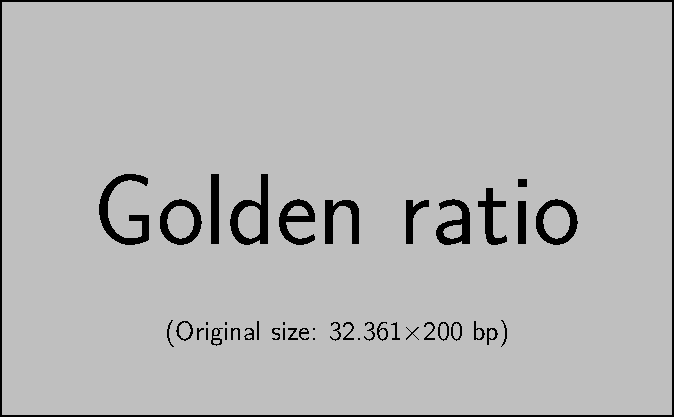
\includegraphics[width=\textwidth]{placeholder_images/example-image-golden.pdf}
    \caption[Timing diagram of a real-time software loop of a \gls{bms}]
    {Timing diagram of a real-time software loop of a \gls{bms}. The integration  of the  \gls{bms} within  the larger  scope of  a master  vehicular controller is not shown}
    \label{fig:timingdiagramBig}
\end{figure}




% Figure from Steve Southward or from plett. Ignore the computational delay
% analytical solution (but not really applicable in state-estimation tasks)
% decoupled
% basic discretisation
% System transition matrix (matrix exponential)
% frequency range
% EPA
% Power input (lack of measurements in current)
% Parameter estimation
% Sampling/quantisation/z-domain/fourier analysis/Pre-conditioning/ZOH
% Sampled systems are also essential in considering Kalman versions
% Can talk in depth about Fwd Euler, Tustin vs matrix exponential approach
% better to perform a vector-update (although certainly it is easy to do scalar
% update)
% Block diagram and stuff
% comparison of approximations
% show some inline minted code, ode45, Ac vs A discrete etc
% modes are decoupled



% \begin{figure}[htb]
%     \begin{algorithmic}[1]

%         \Procedure{SUM}{ $\{x\}$}

%         \State $y\gets0$
%         \For{$i \gets 1 : N^{x}$} \Comment{Time series $\{x\}$ has length $N^{x}$}
%         \State $y\gets y+x(i)$ \Comment{Summing up.}
%         \EndFor

%         \State \textbf{return}  $y$
%         \EndProcedure
%     \end{algorithmic}
%     \caption[Implementation of a algorithm for calculating a sum.]{Implementation of a algorithm for calculating a sum.}
%     \label{fig:algorithm1}
% \end{figure}

% The \textproc{Sum} algorithm shows blah blah blah
% % inside algorithm,
% % cases environment, displayed equations, chapter wise algorithm numbering
% % referencing function names in small caps

% % https://tex.stackexchange.com/questions/113719/cleveref-fails-to-reference-algorithms

% % https://tex.stackexchange.com/questions/110412/numbering-in-algorithmicx
% % https://tex.stackexchange.com/questions/65993/algorithm-numbering

% % https://tex.stackexchange.com/questions/203713/how-can-i-typeset-function-names-as-they-appear-in-algorithmic-environments
% % https://tex.stackexchange.com/questions/100346/typesetting-listofalgorithms-like-listoffigures-and-listoftables-using-titletoc
% % https://tex.stackexchange.com/questions/30363/how-do-i-define-a-new-command-in-algorithmicx

% % https://tex.stackexchange.com/questions/67908/customizing-the-algorithmic-package-break-and-loop-labels

% % https://tex.stackexchange.com/questions/69449/avoid-putting-statements-on-the-same-line-with-algorithmicx

% % \usepackage{float}
% % \newfloat{algorithm}{t}{lop}
% % Add \floatname{algorithm}{Algorithm} to capitalise the float name
